\clearpage
//%%%%%%%%%%%%%%%%%%%%%%%%%%%%%%%%%%%%%%%%%%%%%%%%%%%%%%%%%%%%%%%%%%%%%%%%%%%%%%%%%%%%%%%%%%%%%%%%%%%%%%%%%%%%%%%%%%%%%%%%%%%%%%%%%%%%%%%%%%%%%%%%%%

\section{M-QAM Receiver}\label{lib:homodyneRx}

\begin{tcolorbox}	
	\begin{tabular}{p{2.75cm} p{0.2cm} p{10.5cm}} 	
		\textbf{Header File}   &:& m\_qam\_receiver.h \\
		\textbf{Source File}   &:& m\_qam\_receiver.cpp \\
        \textbf{Version}       &:& 20190403 (\emph{Lucas Leitao})\\
	\end{tabular}
\end{tcolorbox}

This block simulates the reception, all the signal processing and demodulation of an optical
signal (which is the input signal of the system) and outputs a binary signal
corresponding to the reconstructed transmitted bitstream.
 A simplified schematic representation of this block is shown in
figure
\ref{fig:homodyneRx_simple}.

\begin{figure}[h]
	\centering
	\includegraphics[width=0.5\textwidth]{../lib/m_qam_receiver/figures/homodyneRx_simple.pdf}
	\caption{Simplified model of the MQAM
	receiver}\label{fig:homodyneRx_simple}
\end{figure}

\subsection*{Functional description}

This block accepts one optical input signal and outputs one binary signal that
corresponds to the decoded information transmitted in the input signal. It is a
complex
block (as it can be seen from figure \ref{fig:homodyneRx_blocks}) made up of
several simpler blocks whose description can be found in the
\textit{lib} repository. Unlike the block in \ref{lib:mqamRx}, this block does
not include the local oscillator.

\begin{figure}[h]
	\centering
	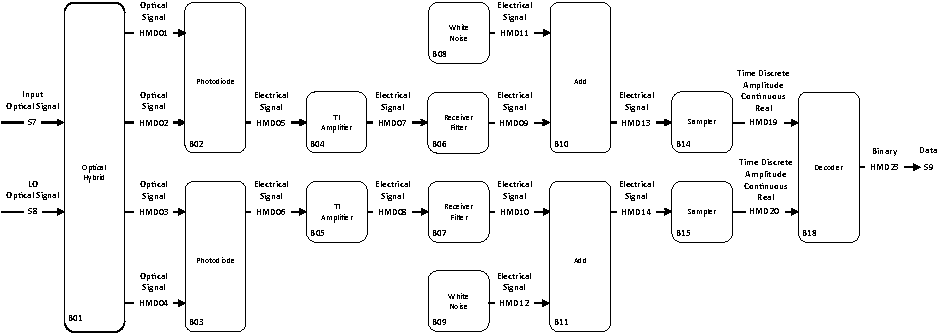
\includegraphics[width=\textwidth]{../lib/m_qam_receiver/figures/homodyneRx_blocks.pdf}
	\caption{Schematic representation of the block homodyne
	receiver.}\label{fig:homodyneRx_blocks}
\end{figure}

\subsection*{Input parameters}

This block input parameters that can be manipulated by the user in
order to change the configuration of the receiver. Each parameter is changed by
calling a
particular function. In the following table
(Table~\ref{tab:homodyneRx_params}) the input parameters and corresponding
functions are
summarized.
%
\begin{table}[h]
	\begin{center}
		\begin{tabular}{| m{3,2cm} | m{6,2cm} |  m{2,2cm} | m{4cm} | }
			\hline
			\textbf{Input parameters} & \textbf{Function} & \textbf{Type} &
			\textbf{Accepted values} \\ \hline
%			IQ amplitudes & setIqAmplitudes & Vector of coordinate points in the I-Q
%			plane & \textbf{Example} for a 4-QAM mapping: \{ \{ 1.0, 1.0 \}, \{ -1.0,
%			1.0 \}, \{ -1.0, -1.0 \}, \{ 1.0, -1.0 \} \} \\ \hline
%			Local oscillator power (in dBm) & setLocalOscillatorOpticalPower\_dBm &
%			double(t\_real) & Any double greater than zero\\ \hline
%			Local oscillator phase & setLocalOscillatorPhase & double(t\_real) & Any
%			double greater than zero\\ \hline
%			Responsivity of the photodiodes & setResponsivity & double(t\_real)
%			&$\in$ [0,1] \\ \hline
%			Amplification (of the TI amplifier) & setAmplification & double(t\_real)
%			& Positive real number\\ \hline
%			Noise amplitude (introduced by the TI amplifier) & setNoiseAmplitude &
%			double(t\_real) & Real number greater than zero \\ \hline
%			Samples to skipe & setSamplesToSkip & int(t\_integer) &  \\ \hline
%			Save internal signals & setSaveInternalSignals & bool & True or False\\
%			\hline
%			Sampling period & setSamplingPeriod & double & Given by
%			\textit{symbolPeriod}/\textit{samplesPerSymbol}\\
%			\hline
		\end{tabular}
		\caption{List of input parameters of the block MQAM receiver}
		\label{tab:homodyneRx_params}
	\end{center}
\end{table}
%
%\pagebreak

\subsection*{Methods}

%HomodyneReceiver(vector$<$Signal *$>$ \&inputSignal, vector$<$Signal *$>$
%\&outputSignal) (\textbf{constructor})
%\bigbreak
%void setIqAmplitudes(vector$<$t\_iqValues$>$ iqAmplitudesValues)
%\bigbreak
%vector$<$t\_iqValues$>$ const getIqAmplitudes(void)
%\bigbreak
%void setLocalOscillatorSamplingPeriod(double sPeriod)
%\bigbreak
%void setLocalOscillatorOpticalPower(double opticalPower)
%\bigbreak
%void setLocalOscillatorOpticalPower\_dBm(double opticalPower\_dBm)
%\bigbreak
%void setLocalOscillatorPhase(double lOscillatorPhase)
%\bigbreak
%void setLocalOscillatorOpticalWavelength(double lOscillatorWavelength)
%\bigbreak
%void setSamplingPeriod(double sPeriod)
%\bigbreak
%void  setResponsivity(t\_real Responsivity)
%\bigbreak
%void setAmplification(t\_real Amplification)
%\bigbreak
%void setNoiseAmplitude(t\_real NoiseAmplitude)
%\bigbreak
%void setImpulseResponseTimeLength(int impResponseTimeLength)
%\bigbreak
%void setFilterType(PulseShaperFilter fType)
%\bigbreak
%void setRollOffFactor(double rOffFactor)
%\bigbreak
%void setClockPeriod(double per)
%\bigbreak
%void setSamplesToSkip(int sToSkip)
%
%\pagebreak

\subsection*{Input Signals}

\subparagraph*{Number:} 2

\subparagraph*{Type:} Optical signal

\subsection*{Output Signals}

\subparagraph*{Number:} 1

\subparagraph*{Type:} Binary signal

\subsection*{Example}

\subsection*{Sugestions for future improvement}

//%%%%%%%%%%%%%%%%%%%%%%%%%%%%%%%%%%%%%%%%%%%%%%%%%%%%%%%%%%%%%%%%%%%%%%%%%%%%%%%%
//%%%%%%%%%%%%%%%%%%%%%%%%%%%%%%%%%%%%%%%%%%%%%%%%%%%%%%%%%%%%%%%%%%%%%%%%%%%%%%%%
//%%%%%%%%%%%%%%%%%%%%%%%%%%%%%%%%%%%%%%%%%%%%%%%%%%%%%%%%%%%%%%%%%%%%%%%%%%%%%%%%

 \subsection*{\textbf{Version 20190403}}

This super block simulates the reception, all the processing and demodulation of an optical
signal.\\
Inside this super blocks, we have important blocks, such as the Ti Amplifier and the Eletrical Filter.
(Noise simulation and analysis is also important in this block
It outputs a binary signal corresponding to the reconstructed transmitted bitstream.
A simplified schematic representation of this block is shown in
figure \ref{fig:homodyneRx_simple}.

\begin{figure}[H]
	\centering
	\includegraphics[width=0.5\textwidth]{../lib/m_qam_receiver/figures/homodyneRx_simple.pdf}
	\caption{Simplified model of the MQAM receiver}\label{fig:homodyneRx_simple}
\end{figure}
\subsection*{Input Signals}

\subparagraph*{Number:} 2

\subparagraph*{Type:} Optical signal

\subsection*{Output Signals}

\subparagraph*{Number:} 1

\subparagraph*{Type:} Binary signal

\subsection*{Input parameters}

Besides the input signals described above, this "super block" has different input parameters
that can be later changed using the methods summarized in the "Functions to set parameters" section below.

\subsection*{Methods}


\begin{enumerate}
\item Block Declaration and Initialization
             \begin{itemize}
                 \item MQamReceiver(initializer\_list$<$Signal *$>$ \&inputSig, initializer\_list$<$Signal *$>$ \&outputSig)
                 \item void initialize(void)
	             \item bool runBlock(void)
	             \item bool firstTime(true)
             \end{itemize}
\item Functions to set parameters
             \begin{itemize}
            %Photodiodes config\\
                \item void setPhotodiodesResponsivity(t\_real Responsivity)\\
            %TI Amplifier config\\
                \item void setGain(t\_real gain)
                \item void setAmplifierInputNoisePowerSpectralDensity(t\_real NoiseSpectralDensity)
                \item void setTiAmplifierFilterType(Filter fType)
                \item void setTiAmplifierCutoffFrequency(double ctfFreq)
                \item void setTiAmplifierImpulseResponseTimeLength\_symbolPeriods(int irl)
                \item void setElectricalFilterImpulseResponse(vector$<$t\_real$>$ ir)
                \item void setElectricalImpulseResponseFilename(string fName)
                \item void setElectricalSeeBeginningOfImpulseResponse(bool sBeginningOfImpulseResponse) \\
            %General Noise\\
                \item void setNoiseSamplingPeriod(t\_real SamplingPeriod)
                \item void setNoiseSymbolPeriod(t\_real nSymbolPeriod) \\
            %Thermal Noise\\
                \item voidsetThermalNoiseSpectralDensity(t\_real NoiseSpectralDensity)
                \item void setThermalNoisePower(t\_real NoiseSpectralDensity)
                \item void setThermalConstantPower(bool cp)
                \item void setSeeds(array$<$int, 2$>$ noiseSeeds)
                \item void setSeedType(SeedType seedType)\\
            %Pulse Shaper\\
                \item void setImpulseResponseTimeLength(int impResponseTimeLength)
                \item void setFilterType(pulse\_shapper\_filter\_type fType)
                \item void setRollOffFactor(double rOffFactor)
                \item void usePassiveFilterMode(bool pFilterMode)
                \item void setRrcNormalizeEnergy(bool ne)
                \item void setMFImpulseResponseFilename(string fName)
                \item void setMFSeeBeginningOfImpulseResponse(bool sBeginningOfImpulseResponse)
                \item double const getMFSeeBeginningOfImpulseResponse(void)\\
            %Sampler\\
                \item void setSamplesToSkip(int sToSkip)\\
            %Decoder\\
                \item void setIqAmplitudes(vector$<$t\_iqValues$>$ iqAmplitudesValues)\\
             \end{itemize}
\item Functions to get parameters
             \begin{itemize}
                \item t\_real getGain(void)
                \item t\_real getAmplifierInputNoisePowerSpectralDensity(void)
                \item double const getElectricalSeeBeginningOfImpulseResponse(void)
                \item vector$<$t\_iqValues$>$ const getIqAmplitudes(void)
             \end{itemize}
\end{enumerate}
\pagebreak
\subsection*{Functional description}

This block accepts one optical signal and a the "Receiver Oscillator Output" as inputs. It outputs one binary signal that corresponds to the decoded information transmitted in the input signal. It is a complex
block (as it can be seen from figure \ref{fig:homodyneRx_blocks}) made up of
several simpler blocks.

\begin{figure}[H]
	\centering
	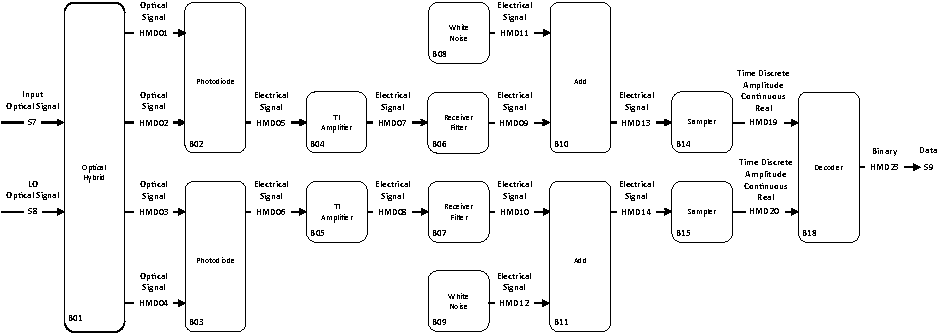
\includegraphics[width=\textwidth]{../lib/m_qam_receiver/figures/homodyneRx_blocks.pdf}
	\caption{Schematic representation of the block homodyne
	receiver.}\label{fig:homodyneRx_blocks}
\end{figure}
A detailed functional description of each block, can be found within this chapter (in different sections).
\subsection*{Examples}
\subsection*{Receiver Sensitivity (Thermal Noise) Test}
To test the thermal noise effect on the receiver sensitivity, we first consider, as a reference, the case of when the received signal is a QPSK, with no thermal noise.\\
For this case, the White noise amplitude will be zero, so, it is expected BER=0
\begin{figure}[H]
	\centering
	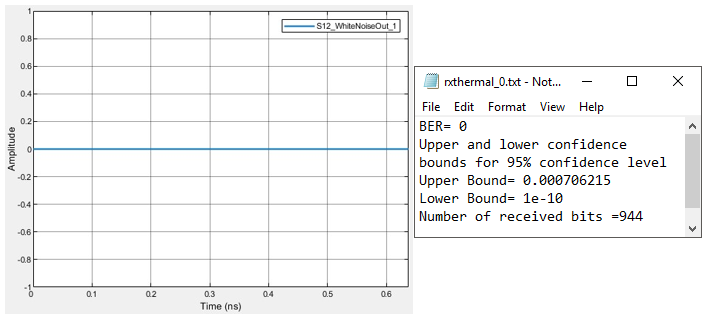
\includegraphics[scale=0.75]{./lib/m_qam_receiver/figures/whiteN0}
	\caption{WhiteNoise Amplitude and consequent BER.}\label{whiteN0}
\end{figure}
By changing the "NoiseSpectralDensityr" value to $1e-3$, we are changing the white noise amplitude. In consequence, the noise power will increase , so as the BER, as shown below:
\begin{figure}[H]
	\centering
	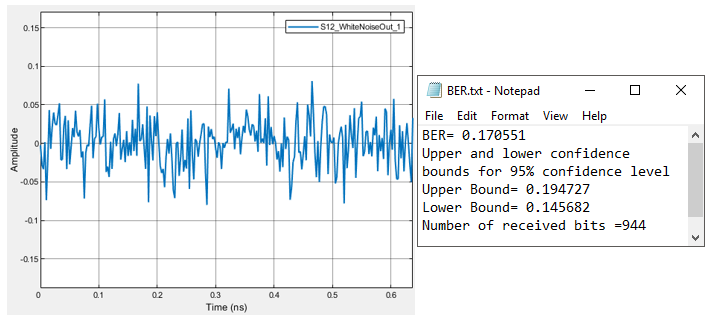
\includegraphics[scale=0.75]{./lib/m_qam_receiver/figures/whiteN10}
	\caption{WhiteNoise Amplitude and consequent BER.}\label{whiteN10}
\end{figure}
It is then possible to conclude that with a higher thermal noise, the receiver sensitivity will get worst, since the lowest received signal power must be increased in order to have a correct demodulation.
\subsection*{Ti Amplifier Gain Test}
The "Ti Amplifier" block, is critical in terms of noise at the receiver side. It must add to the system the minimum noise. The other noise sources, like thermal or quantic, are irrelevant if the the amplifier has a good gain and adds practically no noise. To test that, it is added thermal noise ($rxThermalNoisePower=7e-4$) to the simulation.\\
(The simulation was not completed due to some problems not solved until this day)


\subsection*{Ti Amplifier Bandwidth Test}
By changing the bandwidth of the "Ti Amplifier" Block, it is possible to check its effect on the decoded information.
As a reference value, we can consider the QPSK signal with a signal period of $2e-11$, so using a 50GHz bandwidth filter, the signal out of the Ti Amplfifier will just be a delayed version of the input signal.
\begin{figure}[H]
	\centering
	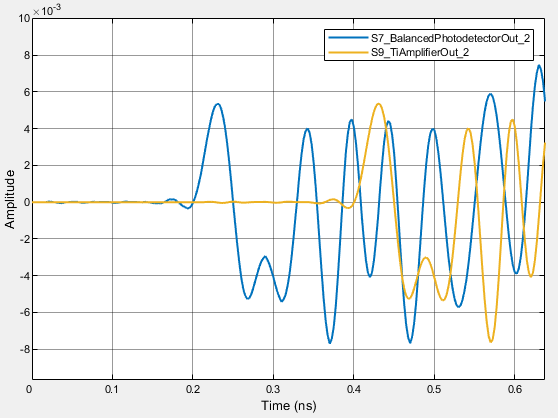
\includegraphics[scale=0.75]{./lib/m_qam_receiver/figures/tiamp1}
	\caption{Ti Amplifier (50GHz) - Input/Out signals}\label{tiamp1}
\end{figure}
If the bandwidth is shortened (to 10GHz, for example), the output signal, will then be distorted, since some of the information is "filtered".
 \begin{figure}[H]
	\centering
	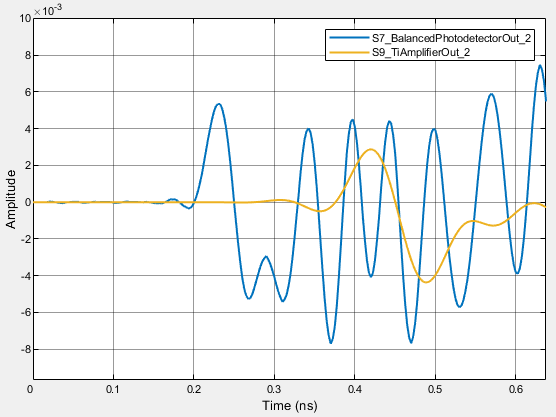
\includegraphics[scale=0.75]{./lib/m_qam_receiver/figures/tiamp2}
	\caption{Ti Amplifier (10GHz) - Input/Out signals}\label{tiamp2}
\end{figure}

\subsection*{Eletrical Filter Test}
Both in the transmitter/receiver side, were tested 2 different filters shapers.
Considering that a root raised cosine filter is used in the transmitter, if the same filter is used in the reception, then we can see that ISI in the optimum sampling instant is zero (because by multiplying two root raised cosine filter, a raised cosine filter is obtained, which main characteristic is having the zero ISI in the optimum sampling instant).
 \begin{figure}[H]
	\centering
	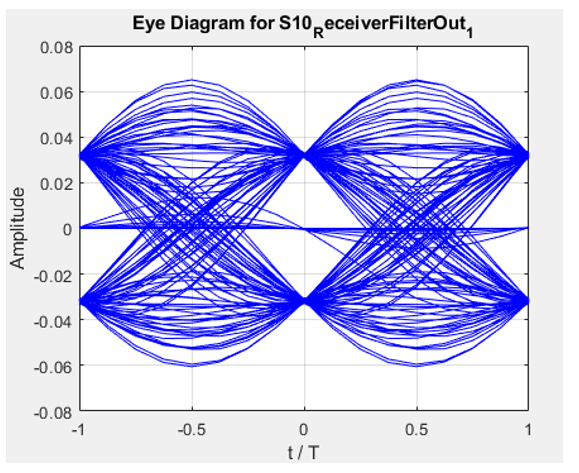
\includegraphics[scale=0.75]{./lib/m_qam_receiver/figures/rootroot}
	\caption{Eletrical Filter Output (Eye Diagram) and BER file }\label{root}
\end{figure}

As expected, through the Eye's diagram, we confirm the $ISI=0$. \\

Considering that a raised cosine filter is used in the transmitter, if the same filter is used in the reception, the ISI in the optimum sampling instant is different than zero (because the filter multiplication will give a squared raised cosine filter, that has ISI different than zero in the optimum sampling instant).
 \begin{figure}[H]
	\centering
	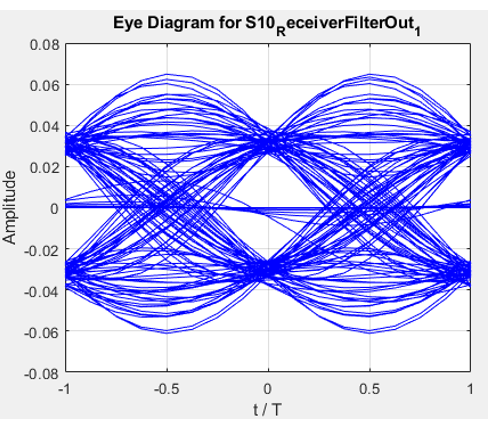
\includegraphics[scale=0.75]{./lib/m_qam_receiver/figures/raisedraised}
	\caption{Eletrical Filter Output (Eye Diagram) and BER file }\label{raised}
\end{figure}
The simulated result corroborates what is written above\\
\subsection*{Different Constellations and associated BER Test}
This simulation detailed description is in the "M-QAM Transmitter Block".

\subsection*{Open Issues}
\begin{itemize}
    \item This "M-QAM Receiver" block should be after the Transmission Block.
    \item A problem with the "Vizualizer.m" makes impossible to analyse the different signal in the frequency domain.
    \item The Decoding process is not performing well when decoding a 16QAM signal (didn't found the solution yet)
\end{itemize}
\subsection*{Future Improvements}
\begin{itemize}
    \item Improve the Code "readability" (just by deleting unnecessary commentaries)
    \item Improve the "Decoder" versatility, by enabling it to decode a wider range of constellations and codifications
    \item Some Block input parameters are defined in the block header file (it would be easir to simulate the system, if all system parameters were accessible in the main file).
\end{itemize} 